\documentclass{article}

\usepackage{noweb}
\noweboptions{smallcode,longchunks}

\usepackage[a4paper,margin=1in]{geometry}

\usepackage{colortbl}
\usepackage[colorlinks=true]{hyperref}
\usepackage{graphicx}

% Define a handy paragraph opener
\newcommand{\hi}[1]{\noindent {\bf #1}}

% Remove noweb page break penalty
\def\nwendcode{\endtrivlist \endgroup}
\let\nwdocspar=\par

\title{Jargo Simulation Interface\footnote{\url{https://github.com/jargors/Simulation-Interface}}}
\author{James J. Pan\\
  \small{\href{mailto:jamesjpan@outlook.com}{jamesjpan@outlook.com}}
}

\begin{document}
\maketitle
\pagestyle{noweb}

\tableofcontents

\section{Introduction}
\label{sec:introduction}
Jargo's simulation interface provides a way for Jargo clients to interact with
the Jargo simulated world (Figure~\ref{fig:interface-fig}). The interface
exposes only the subset of Jargo's storage interface API that a client would
possibly have access to in the real world, including querying and submitting
server routes and schedules.  The simulation interface is developed using the
Noweb\footnote{\url{https://www.cs.tufts.edu/~nr/noweb/}} literate
programming\footnote{\url{http://literateprogramming.com/}} tool.  This file
({\tt{}src/SimulationInterface.nw}) is the source for the documentation
({\tt{}doc/SimulationInterface.tex}) and the Java code
({\tt{}SimulationInterface.java})\footnote{See the {\tt{}Makefile} for build
details.}.

\begin{figure}[h]
\centering
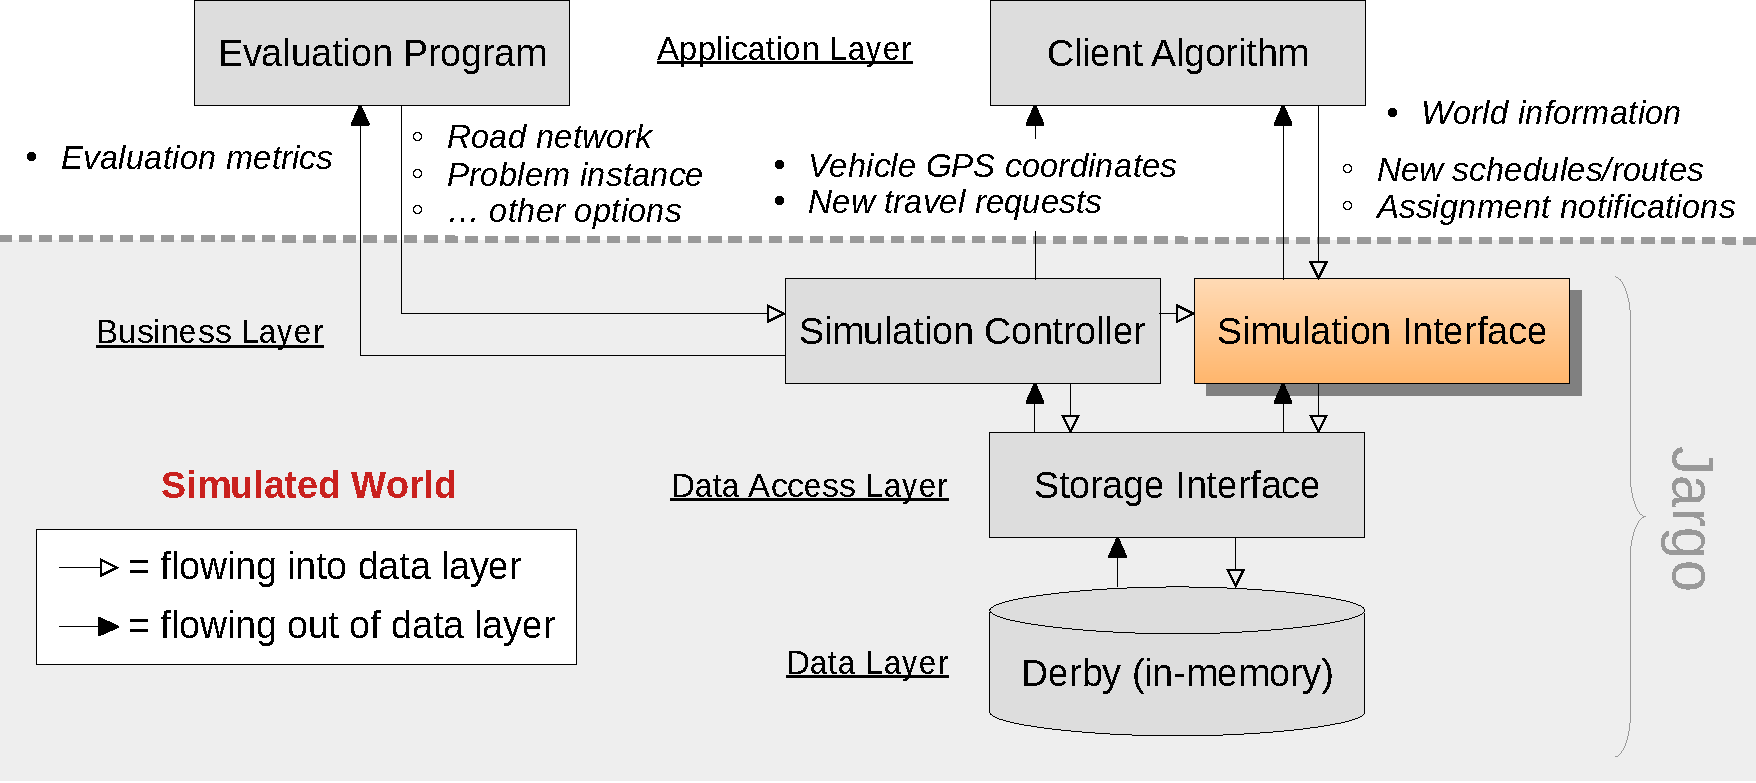
\includegraphics[width=150mm]{src/fig/interface-fig}
\caption{Simulation interface within the Jargo stack.}
\label{fig:interface-fig}
\end{figure}

\section{Implementation Overview}
\label{sec:implementation-overview}
\nwfilename{src/SimulationInterface.nw}\nwbegincode{1}\sublabel{NW3Bji2p-2qVXZY-1}\nwmargintag{{\nwtagstyle{}\subpageref{NW3Bji2p-2qVXZY-1}}}\moddef{SimulationInterface.java~{\nwtagstyle{}\subpageref{NW3Bji2p-2qVXZY-1}}}\endmoddef\nwnotused{SimulationInterface.java}
  \LA{}SimulationInterface.java preamble~{\nwtagstyle{}\subpageref{NW3Bji2p-1Ogd8c-1}}\RA{}
  \LA{}\code{}SimulationInterface\edoc{} definition~{\nwtagstyle{}\subpageref{NW3Bji2p-2ph1Ov-1}}\RA{}
\nwendcode{}\nwbegindocs{2}\nwdocspar

\subsection{Preamble}
\label{sec:preamble}
The preamble declares the package and imports dependencies.
\nwenddocs{}\nwbegincode{3}\sublabel{NW3Bji2p-1Ogd8c-1}\nwmargintag{{\nwtagstyle{}\subpageref{NW3Bji2p-1Ogd8c-1}}}\moddef{SimulationInterface.java preamble~{\nwtagstyle{}\subpageref{NW3Bji2p-1Ogd8c-1}}}\endmoddef\nwalsodefined{\\{NW3Bji2p-1Ogd8c-2}}\nwused{\\{NW3Bji2p-2qVXZY-1}}
package com.github.jargors;
\nwendcode{}\nwbegindocs{4}\nwdocspar
\nwenddocs{}\nwbegincode{5}\sublabel{NW3Bji2p-1Ogd8c-2}\nwmargintag{{\nwtagstyle{}\subpageref{NW3Bji2p-1Ogd8c-2}}}\moddef{SimulationInterface.java preamble~{\nwtagstyle{}\subpageref{NW3Bji2p-1Ogd8c-1}}}\plusendmoddef
import com.github.jargors.StorageInterface;
import java.util.function.Supplier;
import java.time.LocalDateTime;
\nwendcode{}\nwbegindocs{6}\nwdocspar

\subsection{Class Definition}
\label{sec:class-definition}
The {\tt{}SimulationInterface} class consists of member variables, a constructor, and public
and private methods, just like any other Java class.
\nwenddocs{}\nwbegincode{7}\sublabel{NW3Bji2p-2ph1Ov-1}\nwmargintag{{\nwtagstyle{}\subpageref{NW3Bji2p-2ph1Ov-1}}}\moddef{\code{}SimulationInterface\edoc{} definition~{\nwtagstyle{}\subpageref{NW3Bji2p-2ph1Ov-1}}}\endmoddef\nwused{\\{NW3Bji2p-2qVXZY-1}}
public class SimulationInterface \{
  \LA{}\code{}SimulationInterface\edoc{} member variables~{\nwtagstyle{}\subpageref{NW3Bji2p-kPmHg-1}}\RA{}
  \LA{}\code{}SimulationInterface\edoc{} constructor~{\nwtagstyle{}\subpageref{NW3Bji2p-1BYMMV-1}}\RA{}
  \LA{}\code{}SimulationInterface\edoc{} public methods~{\nwtagstyle{}\subpageref{NW3Bji2p-48YU8C-1}}\RA{}
  \LA{}\code{}SimulationInterface\edoc{} private methods~{\nwtagstyle{}\subpageref{NW3Bji2p-3pxn9j-1}}\RA{}
\}
\nwendcode{}\nwbegindocs{8}\nwdocspar

\subsection{Member Variables}
\label{sec:member-variables}
We define a {\tt{}StorageInterface} and a container for the simulation world time.
\nwenddocs{}\nwbegincode{9}\sublabel{NW3Bji2p-kPmHg-1}\nwmargintag{{\nwtagstyle{}\subpageref{NW3Bji2p-kPmHg-1}}}\moddef{\code{}SimulationInterface\edoc{} member variables~{\nwtagstyle{}\subpageref{NW3Bji2p-kPmHg-1}}}\endmoddef\nwused{\\{NW3Bji2p-2ph1Ov-1}}
private StorageInterface storage;
private int world_time = 0;
\nwindexdefn{storage}{storage}{NW3Bji2p-kPmHg-1}\nwindexdefn{world{\char95}time}{world:untime}{NW3Bji2p-kPmHg-1}\eatline
\nwidentdefs{\\{{storage}{storage}}\\{{world{\char95}time}{world:untime}}}\nwendcode{}\nwbegindocs{10}\nwdocspar
\subsection{Constructor}
\label{sec:constructor}
The storage interface is set in the constructor.
\nwenddocs{}\nwbegincode{11}\sublabel{NW3Bji2p-1BYMMV-1}\nwmargintag{{\nwtagstyle{}\subpageref{NW3Bji2p-1BYMMV-1}}}\moddef{\code{}SimulationInterface\edoc{} constructor~{\nwtagstyle{}\subpageref{NW3Bji2p-1BYMMV-1}}}\endmoddef\nwused{\\{NW3Bji2p-2ph1Ov-1}}
public SimulationInterface(StorageInterface src) \{
  storage = src;
\}
\nwidentuses{\\{{storage}{storage}}}\nwindexuse{storage}{storage}{NW3Bji2p-1BYMMV-1}\nwendcode{}\nwbegindocs{12}\nwdocspar

\section{Public Methods}
\label{sec:public-methods}
\hi{General Methods.}
\nwenddocs{}\nwbegincode{13}\sublabel{NW3Bji2p-48YU8C-1}\nwmargintag{{\nwtagstyle{}\subpageref{NW3Bji2p-48YU8C-1}}}\moddef{\code{}SimulationInterface\edoc{} public methods~{\nwtagstyle{}\subpageref{NW3Bji2p-48YU8C-1}}}\endmoddef\nwalsodefined{\\{NW3Bji2p-48YU8C-2}\\{NW3Bji2p-48YU8C-3}}\nwused{\\{NW3Bji2p-2ph1Ov-1}}
\LA{}Set/get simulation world time~{\nwtagstyle{}\subpageref{NW3Bji2p-3SIXWk-1}}\RA{}
\nwendcode{}\nwbegindocs{14}\nwdocspar
\hi{Write Methods.}
\nwenddocs{}\nwbegincode{15}\sublabel{NW3Bji2p-48YU8C-2}\nwmargintag{{\nwtagstyle{}\subpageref{NW3Bji2p-48YU8C-2}}}\moddef{\code{}SimulationInterface\edoc{} public methods~{\nwtagstyle{}\subpageref{NW3Bji2p-48YU8C-1}}}\plusendmoddef
\LA{}Update server route~{\nwtagstyle{}\subpageref{NW3Bji2p-4VFddh-1}}\RA{}
\LA{}Update server add to schedule~{\nwtagstyle{}\subpageref{NW3Bji2p-y828a-1}}\RA{}
\LA{}Update server remove from schedule~{\nwtagstyle{}\subpageref{NW3Bji2p-lMiTm-1}}\RA{}
\nwendcode{}\nwbegindocs{16}\nwdocspar
\hi{Read Methods.}
\nwenddocs{}\nwbegincode{17}\sublabel{NW3Bji2p-48YU8C-3}\nwmargintag{{\nwtagstyle{}\subpageref{NW3Bji2p-48YU8C-3}}}\moddef{\code{}SimulationInterface\edoc{} public methods~{\nwtagstyle{}\subpageref{NW3Bji2p-48YU8C-1}}}\plusendmoddef
\LA{}Query vertex~{\nwtagstyle{}\subpageref{NW3Bji2p-4IfXsG-1}}\RA{}
\LA{}Query edge~{\nwtagstyle{}\subpageref{NW3Bji2p-1E2aru-1}}\RA{}
\LA{}Query ridesharing user~{\nwtagstyle{}\subpageref{NW3Bji2p-3isdeu-1}}\RA{}
\LA{}Query active server locations~{\nwtagstyle{}\subpageref{NW3Bji2p-3UaQCb-1}}\RA{}
\LA{}Query routes~{\nwtagstyle{}\subpageref{NW3Bji2p-1AprqI-1}}\RA{}
\LA{}Query schedules~{\nwtagstyle{}\subpageref{NW3Bji2p-3yA8FQ-1}}\RA{}
\LA{}Query current load~{\nwtagstyle{}\subpageref{NW3Bji2p-aKbeg-1}}\RA{}
\nwendcode{}\nwbegindocs{18}\nwdocspar

\subsection{General Methods}
\label{sec:general-methods}

\subsubsection{{\tt{}\protect\nosublabel{NW3Bji2p-48YU8C-3-u7}\protect\nwindexuse{setSimulationWorldTime}{setSimulationWorldTime}{NW3Bji2p-3SIXWk-1}setSimulationWorldTime}(1)}
We depend on the controller to tell the simulation interface about the current
world time.
\nwenddocs{}\nwbegincode{19}\sublabel{NW3Bji2p-3SIXWk-1}\nwmargintag{{\nwtagstyle{}\subpageref{NW3Bji2p-3SIXWk-1}}}\moddef{Set/get simulation world time~{\nwtagstyle{}\subpageref{NW3Bji2p-3SIXWk-1}}}\endmoddef\nwalsodefined{\\{NW3Bji2p-3SIXWk-2}}\nwused{\\{NW3Bji2p-48YU8C-1}}
public void setSimulationWorldTime(int t) \{
  world_time = t;
\}
\nwindexdefn{setSimulationWorldTime}{setSimulationWorldTime}{NW3Bji2p-3SIXWk-1}\eatline
\nwidentdefs{\\{{setSimulationWorldTime}{setSimulationWorldTime}}}\nwidentuses{\\{{world{\char95}time}{world:untime}}}\nwindexuse{world{\char95}time}{world:untime}{NW3Bji2p-3SIXWk-1}\nwendcode{}\nwbegindocs{20}\nwdocspar
\subsubsection{{\tt{}\protect\nwindexuse{getSimulationWorldTime}{getSimulationWorldTime}{NW3Bji2p-3SIXWk-2}getSimulationWorldTime}(0)}
\nwenddocs{}\nwbegincode{21}\sublabel{NW3Bji2p-3SIXWk-2}\nwmargintag{{\nwtagstyle{}\subpageref{NW3Bji2p-3SIXWk-2}}}\moddef{Set/get simulation world time~{\nwtagstyle{}\subpageref{NW3Bji2p-3SIXWk-1}}}\plusendmoddef
public int getSimulationWorldTime() \{
  return world_time;
\}
\nwindexdefn{getSimulationWorldTime}{getSimulationWorldTime}{NW3Bji2p-3SIXWk-2}\eatline
\nwidentdefs{\\{{getSimulationWorldTime}{getSimulationWorldTime}}}\nwidentuses{\\{{world{\char95}time}{world:untime}}}\nwindexuse{world{\char95}time}{world:untime}{NW3Bji2p-3SIXWk-2}\nwendcode{}\nwbegindocs{22}\nwdocspar
\subsection{Write Methods}
\label{sec:write-methods}

\subsubsection{{\tt{}\protect\nwindexuse{updateServerRoute}{updateServerRoute}{NW3Bji2p-4VFddh-1}updateServerRoute}(3)}
\nwenddocs{}\nwbegincode{23}\sublabel{NW3Bji2p-4VFddh-1}\nwmargintag{{\nwtagstyle{}\subpageref{NW3Bji2p-4VFddh-1}}}\moddef{Update server route~{\nwtagstyle{}\subpageref{NW3Bji2p-4VFddh-1}}}\endmoddef\nwused{\\{NW3Bji2p-48YU8C-2}}
public void updateServerRoute(int sid, int[] route, int[] sched) \{
  storage.DBUpdateServerRoute(sid, route, sched);
\}
\nwindexdefn{updateServerRoute}{updateServerRoute}{NW3Bji2p-4VFddh-1}\eatline
\nwidentdefs{\\{{updateServerRoute}{updateServerRoute}}}\nwidentuses{\\{{storage}{storage}}}\nwindexuse{storage}{storage}{NW3Bji2p-4VFddh-1}\nwendcode{}\nwbegindocs{24}\nwdocspar
\subsubsection{{\tt{}\protect\nwindexuse{updateServerAddToSchedule}{updateServerAddToSchedule}{NW3Bji2p-y828a-1}updateServerAddToSchedule}(4)}
\nwenddocs{}\nwbegincode{25}\sublabel{NW3Bji2p-y828a-1}\nwmargintag{{\nwtagstyle{}\subpageref{NW3Bji2p-y828a-1}}}\moddef{Update server add to schedule~{\nwtagstyle{}\subpageref{NW3Bji2p-y828a-1}}}\endmoddef\nwused{\\{NW3Bji2p-48YU8C-2}}
public void updateServerAddToSchedule(
    int sid, int[] route, int[] sched, int[] rid) \{
  storage.DBUpdateServerAddToSchedule(sid, route, sched, rid);
\}
\nwindexdefn{updateServerAddToSchedule}{updateServerAddToSchedule}{NW3Bji2p-y828a-1}\eatline
\nwidentdefs{\\{{updateServerAddToSchedule}{updateServerAddToSchedule}}}\nwidentuses{\\{{storage}{storage}}}\nwindexuse{storage}{storage}{NW3Bji2p-y828a-1}\nwendcode{}\nwbegindocs{26}\nwdocspar
\subsubsection{{\tt{}\protect\nwindexuse{updateServerRemoveFromSchedule}{updateServerRemoveFromSchedule}{NW3Bji2p-lMiTm-1}updateServerRemoveFromSchedule}(4)}
\nwenddocs{}\nwbegincode{27}\sublabel{NW3Bji2p-lMiTm-1}\nwmargintag{{\nwtagstyle{}\subpageref{NW3Bji2p-lMiTm-1}}}\moddef{Update server remove from schedule~{\nwtagstyle{}\subpageref{NW3Bji2p-lMiTm-1}}}\endmoddef\nwused{\\{NW3Bji2p-48YU8C-2}}
public void updateServerRemoveFromSchedule(
    int sid, int[] route, int[] sched, int[] rid) \{
  storage.DBUpdateServerRemoveFromSchedule(sid, route, sched, rid);
\}
\nwindexdefn{updateServerRemoveFromSchedule}{updateServerRemoveFromSchedule}{NW3Bji2p-lMiTm-1}\eatline
\nwidentdefs{\\{{updateServerRemoveFromSchedule}{updateServerRemoveFromSchedule}}}\nwidentuses{\\{{storage}{storage}}}\nwindexuse{storage}{storage}{NW3Bji2p-lMiTm-1}\nwendcode{}\nwbegindocs{28}\nwdocspar
\subsection{Read Methods}
\label{sec:read-methods}

\subsubsection{{\tt{}\protect\nwindexuse{queryVertex}{queryVertex}{NW3Bji2p-4IfXsG-1}queryVertex}(1)}
\nwenddocs{}\nwbegincode{29}\sublabel{NW3Bji2p-4IfXsG-1}\nwmargintag{{\nwtagstyle{}\subpageref{NW3Bji2p-4IfXsG-1}}}\moddef{Query vertex~{\nwtagstyle{}\subpageref{NW3Bji2p-4IfXsG-1}}}\endmoddef\nwused{\\{NW3Bji2p-48YU8C-3}}
public int[] queryVertex(int v) throws RuntimeException \{
  return storage.DBQueryVertex(v);
\}
\nwindexdefn{queryVertex}{queryVertex}{NW3Bji2p-4IfXsG-1}\eatline
\nwidentdefs{\\{{queryVertex}{queryVertex}}}\nwidentuses{\\{{storage}{storage}}}\nwindexuse{storage}{storage}{NW3Bji2p-4IfXsG-1}\nwendcode{}\nwbegindocs{30}\nwdocspar
\subsubsection{{\tt{}\protect\nwindexuse{queryEdge}{queryEdge}{NW3Bji2p-1E2aru-1}queryEdge}(2)}
\nwenddocs{}\nwbegincode{31}\sublabel{NW3Bji2p-1E2aru-1}\nwmargintag{{\nwtagstyle{}\subpageref{NW3Bji2p-1E2aru-1}}}\moddef{Query edge~{\nwtagstyle{}\subpageref{NW3Bji2p-1E2aru-1}}}\endmoddef\nwused{\\{NW3Bji2p-48YU8C-3}}
public int[] queryEdge(int v1, int v2) throws RuntimeException \{
  return storage.DBQueryEdge(v1, v2);
\}
\nwindexdefn{queryEdge}{queryEdge}{NW3Bji2p-1E2aru-1}\eatline
\nwidentdefs{\\{{queryEdge}{queryEdge}}}\nwidentuses{\\{{storage}{storage}}}\nwindexuse{storage}{storage}{NW3Bji2p-1E2aru-1}\nwendcode{}\nwbegindocs{32}\nwdocspar
\subsubsection{{\tt{}\protect\nwindexuse{queryServer}{queryServer}{NW3Bji2p-3isdeu-1}queryServer}(1)}
\nwenddocs{}\nwbegincode{33}\sublabel{NW3Bji2p-3isdeu-1}\nwmargintag{{\nwtagstyle{}\subpageref{NW3Bji2p-3isdeu-1}}}\moddef{Query ridesharing user~{\nwtagstyle{}\subpageref{NW3Bji2p-3isdeu-1}}}\endmoddef\nwalsodefined{\\{NW3Bji2p-3isdeu-2}}\nwused{\\{NW3Bji2p-48YU8C-3}}
public int[] queryServer(int sid) throws RuntimeException \{
  return storage.DBQueryServer(sid);
\}
\nwindexdefn{queryServer}{queryServer}{NW3Bji2p-3isdeu-1}\eatline
\nwidentdefs{\\{{queryServer}{queryServer}}}\nwidentuses{\\{{storage}{storage}}}\nwindexuse{storage}{storage}{NW3Bji2p-3isdeu-1}\nwendcode{}\nwbegindocs{34}\nwdocspar
\subsubsection{{\tt{}\protect\nwindexuse{queryRequest}{queryRequest}{NW3Bji2p-3isdeu-2}queryRequest}(1)}
\nwenddocs{}\nwbegincode{35}\sublabel{NW3Bji2p-3isdeu-2}\nwmargintag{{\nwtagstyle{}\subpageref{NW3Bji2p-3isdeu-2}}}\moddef{Query ridesharing user~{\nwtagstyle{}\subpageref{NW3Bji2p-3isdeu-1}}}\plusendmoddef
public int[] queryRequest(int rid) throws RuntimeException \{
  return storage.DBQueryRequest(rid);
\}
\nwindexdefn{queryRequest}{queryRequest}{NW3Bji2p-3isdeu-2}\eatline
\nwidentdefs{\\{{queryRequest}{queryRequest}}}\nwidentuses{\\{{storage}{storage}}}\nwindexuse{storage}{storage}{NW3Bji2p-3isdeu-2}\nwendcode{}\nwbegindocs{36}\nwdocspar
\subsubsection{{\tt{}\protect\nwindexuse{queryServerLocationsActive}{queryServerLocationsActive}{NW3Bji2p-3UaQCb-1}queryServerLocationsActive}(1)}
\nwenddocs{}\nwbegincode{37}\sublabel{NW3Bji2p-3UaQCb-1}\nwmargintag{{\nwtagstyle{}\subpageref{NW3Bji2p-3UaQCb-1}}}\moddef{Query active server locations~{\nwtagstyle{}\subpageref{NW3Bji2p-3UaQCb-1}}}\endmoddef\nwused{\\{NW3Bji2p-48YU8C-3}}
public int[] queryServerLocationsActive(int t) throws RuntimeException \{
  return storage.DBQueryServerLocationsActive(t);
\}
\nwindexdefn{queryServerLocationsActive}{queryServerLocationsActive}{NW3Bji2p-3UaQCb-1}\eatline
\nwidentdefs{\\{{queryServerLocationsActive}{queryServerLocationsActive}}}\nwidentuses{\\{{storage}{storage}}}\nwindexuse{storage}{storage}{NW3Bji2p-3UaQCb-1}\nwendcode{}\nwbegindocs{38}\nwdocspar
\subsubsection{{\tt{}\protect\nwindexuse{queryRouteRemaining}{queryRouteRemaining}{NW3Bji2p-1AprqI-1}queryRouteRemaining}(2)}
\nwenddocs{}\nwbegincode{39}\sublabel{NW3Bji2p-1AprqI-1}\nwmargintag{{\nwtagstyle{}\subpageref{NW3Bji2p-1AprqI-1}}}\moddef{Query routes~{\nwtagstyle{}\subpageref{NW3Bji2p-1AprqI-1}}}\endmoddef\nwused{\\{NW3Bji2p-48YU8C-3}}
public int[] queryRouteRemaining(int sid, int t) throws RuntimeException \{
  return storage.DBQueryRouteRemaining(sid, t);
\}
\nwindexdefn{queryRouteRemaining}{queryRouteRemaining}{NW3Bji2p-1AprqI-1}\eatline
\nwidentdefs{\\{{queryRouteRemaining}{queryRouteRemaining}}}\nwidentuses{\\{{storage}{storage}}}\nwindexuse{storage}{storage}{NW3Bji2p-1AprqI-1}\nwendcode{}\nwbegindocs{40}\nwdocspar
\subsubsection{{\tt{}\protect\nwindexuse{queryScheduleRemaining}{queryScheduleRemaining}{NW3Bji2p-3yA8FQ-1}queryScheduleRemaining}(2)}
\nwenddocs{}\nwbegincode{41}\sublabel{NW3Bji2p-3yA8FQ-1}\nwmargintag{{\nwtagstyle{}\subpageref{NW3Bji2p-3yA8FQ-1}}}\moddef{Query schedules~{\nwtagstyle{}\subpageref{NW3Bji2p-3yA8FQ-1}}}\endmoddef\nwused{\\{NW3Bji2p-48YU8C-3}}
public int[] queryScheduleRemaining(int sid, int t) throws RuntimeException \{
  return storage.DBQueryScheduleRemaining(sid, t);
\}
\nwindexdefn{queryScheduleRemaining}{queryScheduleRemaining}{NW3Bji2p-3yA8FQ-1}\eatline
\nwidentdefs{\\{{queryScheduleRemaining}{queryScheduleRemaining}}}\nwidentuses{\\{{storage}{storage}}}\nwindexuse{storage}{storage}{NW3Bji2p-3yA8FQ-1}\nwendcode{}\nwbegindocs{42}\nwdocspar
\subsubsection{{\tt{}\protect\nwindexuse{queryCurrentLoad}{queryCurrentLoad}{NW3Bji2p-aKbeg-1}queryCurrentLoad}(2)}
\nwenddocs{}\nwbegincode{43}\sublabel{NW3Bji2p-aKbeg-1}\nwmargintag{{\nwtagstyle{}\subpageref{NW3Bji2p-aKbeg-1}}}\moddef{Query current load~{\nwtagstyle{}\subpageref{NW3Bji2p-aKbeg-1}}}\endmoddef\nwused{\\{NW3Bji2p-48YU8C-3}}
public int[] queryCurrentLoad(int sid, int t) throws RuntimeException \{
  return storage.DBQueryCurrentLoad(sid, t);
\}
\nwindexdefn{queryCurrentLoad}{queryCurrentLoad}{NW3Bji2p-aKbeg-1}\eatline
\nwidentdefs{\\{{queryCurrentLoad}{queryCurrentLoad}}}\nwidentuses{\\{{storage}{storage}}}\nwindexuse{storage}{storage}{NW3Bji2p-aKbeg-1}\nwendcode{}\nwbegindocs{44}\nwdocspar
\section{Private Methods}
\label{sec:private-methods}

\subsection{{\tt{}\protect\nwindexuse{Print}{Print}{NW3Bji2p-3pxn9j-1}Print}(1)}
\nwenddocs{}\nwbegincode{45}\sublabel{NW3Bji2p-3pxn9j-1}\nwmargintag{{\nwtagstyle{}\subpageref{NW3Bji2p-3pxn9j-1}}}\moddef{\code{}SimulationInterface\edoc{} private methods~{\nwtagstyle{}\subpageref{NW3Bji2p-3pxn9j-1}}}\endmoddef\nwused{\\{NW3Bji2p-2ph1Ov-1}}
private void Print(String msg) \{
  System.out.println("[Jargo][SimulationInterface]["+LocalDateTime.now()+"] "+msg);
\}
\nwindexdefn{Print}{Print}{NW3Bji2p-3pxn9j-1}\eatline
\nwidentdefs{\\{{Print}{Print}}}\nwendcode{}

\nwixlogsorted{c}{{\code{}SimulationInterface\edoc{} constructor}{NW3Bji2p-1BYMMV-1}{\nwixu{NW3Bji2p-2ph1Ov-1}\nwixd{NW3Bji2p-1BYMMV-1}}}%
\nwixlogsorted{c}{{\code{}SimulationInterface\edoc{} definition}{NW3Bji2p-2ph1Ov-1}{\nwixu{NW3Bji2p-2qVXZY-1}\nwixd{NW3Bji2p-2ph1Ov-1}}}%
\nwixlogsorted{c}{{\code{}SimulationInterface\edoc{} member variables}{NW3Bji2p-kPmHg-1}{\nwixu{NW3Bji2p-2ph1Ov-1}\nwixd{NW3Bji2p-kPmHg-1}}}%
\nwixlogsorted{c}{{\code{}SimulationInterface\edoc{} private methods}{NW3Bji2p-3pxn9j-1}{\nwixu{NW3Bji2p-2ph1Ov-1}\nwixd{NW3Bji2p-3pxn9j-1}}}%
\nwixlogsorted{c}{{\code{}SimulationInterface\edoc{} public methods}{NW3Bji2p-48YU8C-1}{\nwixu{NW3Bji2p-2ph1Ov-1}\nwixd{NW3Bji2p-48YU8C-1}\nwixd{NW3Bji2p-48YU8C-2}\nwixd{NW3Bji2p-48YU8C-3}}}%
\nwixlogsorted{c}{{Query active server locations}{NW3Bji2p-3UaQCb-1}{\nwixu{NW3Bji2p-48YU8C-3}\nwixd{NW3Bji2p-3UaQCb-1}}}%
\nwixlogsorted{c}{{Query current load}{NW3Bji2p-aKbeg-1}{\nwixu{NW3Bji2p-48YU8C-3}\nwixd{NW3Bji2p-aKbeg-1}}}%
\nwixlogsorted{c}{{Query edge}{NW3Bji2p-1E2aru-1}{\nwixu{NW3Bji2p-48YU8C-3}\nwixd{NW3Bji2p-1E2aru-1}}}%
\nwixlogsorted{c}{{Query ridesharing user}{NW3Bji2p-3isdeu-1}{\nwixu{NW3Bji2p-48YU8C-3}\nwixd{NW3Bji2p-3isdeu-1}\nwixd{NW3Bji2p-3isdeu-2}}}%
\nwixlogsorted{c}{{Query routes}{NW3Bji2p-1AprqI-1}{\nwixu{NW3Bji2p-48YU8C-3}\nwixd{NW3Bji2p-1AprqI-1}}}%
\nwixlogsorted{c}{{Query schedules}{NW3Bji2p-3yA8FQ-1}{\nwixu{NW3Bji2p-48YU8C-3}\nwixd{NW3Bji2p-3yA8FQ-1}}}%
\nwixlogsorted{c}{{Query vertex}{NW3Bji2p-4IfXsG-1}{\nwixu{NW3Bji2p-48YU8C-3}\nwixd{NW3Bji2p-4IfXsG-1}}}%
\nwixlogsorted{c}{{Set/get simulation world time}{NW3Bji2p-3SIXWk-1}{\nwixu{NW3Bji2p-48YU8C-1}\nwixd{NW3Bji2p-3SIXWk-1}\nwixd{NW3Bji2p-3SIXWk-2}}}%
\nwixlogsorted{c}{{SimulationInterface.java}{NW3Bji2p-2qVXZY-1}{\nwixd{NW3Bji2p-2qVXZY-1}}}%
\nwixlogsorted{c}{{SimulationInterface.java preamble}{NW3Bji2p-1Ogd8c-1}{\nwixu{NW3Bji2p-2qVXZY-1}\nwixd{NW3Bji2p-1Ogd8c-1}\nwixd{NW3Bji2p-1Ogd8c-2}}}%
\nwixlogsorted{c}{{Update server add to schedule}{NW3Bji2p-y828a-1}{\nwixu{NW3Bji2p-48YU8C-2}\nwixd{NW3Bji2p-y828a-1}}}%
\nwixlogsorted{c}{{Update server remove from schedule}{NW3Bji2p-lMiTm-1}{\nwixu{NW3Bji2p-48YU8C-2}\nwixd{NW3Bji2p-lMiTm-1}}}%
\nwixlogsorted{c}{{Update server route}{NW3Bji2p-4VFddh-1}{\nwixu{NW3Bji2p-48YU8C-2}\nwixd{NW3Bji2p-4VFddh-1}}}%
\nwixlogsorted{i}{{getSimulationWorldTime}{getSimulationWorldTime}}%
\nwixlogsorted{i}{{Print}{Print}}%
\nwixlogsorted{i}{{queryCurrentLoad}{queryCurrentLoad}}%
\nwixlogsorted{i}{{queryEdge}{queryEdge}}%
\nwixlogsorted{i}{{queryRequest}{queryRequest}}%
\nwixlogsorted{i}{{queryRouteRemaining}{queryRouteRemaining}}%
\nwixlogsorted{i}{{queryScheduleRemaining}{queryScheduleRemaining}}%
\nwixlogsorted{i}{{queryServer}{queryServer}}%
\nwixlogsorted{i}{{queryServerLocationsActive}{queryServerLocationsActive}}%
\nwixlogsorted{i}{{queryVertex}{queryVertex}}%
\nwixlogsorted{i}{{setSimulationWorldTime}{setSimulationWorldTime}}%
\nwixlogsorted{i}{{storage}{storage}}%
\nwixlogsorted{i}{{updateServerAddToSchedule}{updateServerAddToSchedule}}%
\nwixlogsorted{i}{{updateServerRemoveFromSchedule}{updateServerRemoveFromSchedule}}%
\nwixlogsorted{i}{{updateServerRoute}{updateServerRoute}}%
\nwixlogsorted{i}{{world{\char95}time}{world:untime}}%
\nwbegindocs{46}\nwdocspar
\appendix

\section{Appendix: List of Chunks}
\label{ap:list-of-chunks}
\nowebchunks

\section{Appendix: List of Identifiers}
\label{ap:list-of-identifiers}
\nowebindex

\end{document}

\nwenddocs{}
